% -*- mode: fundamental -*-

% ****************************************************************

\chapter{The RISC-V implementation Magritte;\\BSV Combinational Circuits and Finite State Machines}

\markboth{Ch \arabic{chapter}: Introduction (DRAFT)}{\copyrightnotice}

\setcounter{page}{1}
% \renewcommand{\thepage}{\arabic{page}}
\renewcommand{\thepage}{\arabic{chapter}-\arabic{page}}

\label{ch_RISCV_Design_Space}

% ****************************************************************

In this chapter we design Magritte, a hardware CPU implementation that
executes the RISC-V ISA.  Magritte is a simple implementation of
RISC-V---it simply executes one complete RISC-V instruction before
starting on the next one.  In particular, it has no pipelining or
architectural sophistication (we will discuss Fife, a pipelined
implementation, later in this book).

Our design is coded in BSV, a modern, high-level HDL.  The BSV code
for Magritte has strong similarities to code written in C (say) for a
simple functional simulator for RISC-V.  Unlike C code, however, our
BSV code will be compiled to Verilog, and will run on an FPGA (it can
also be synthesized into an ASIC).

% ****************************************************************

\section{Simple Instruction Execution}

From our previous study of the RISC-V ISA, we know that the basic
integer ``architectural state'' of a RISC-V CPU is very simple:

\begin{itemize}

\item A ``program counter'' (PC) indicating the address in memory of
the next instruction to be executed.

\item A ``register file'' consisting of 32 general purpose registers
(GPRs), each containing data.

\end{itemize}

The PC and each register are either 32-bits wide (in the RV32 option
of RISC-V) or 64-bits wide (in the RV64 option).  For simplicity,
we'll focus on RV32 here, but everything we discuss also applies to
RV64.

Executing an instruction involves a few simple steps, illustrated in
Figure~\ref{Fig_Simple_Instr_Exec}:
\begin{figure}[htbp]
  \centerline{\includegraphics[width=6in,angle=0]{ch030_RISCV_Design_Space/Figures/Fig_Simple_Instr_Exec}}
  \caption{\label{Fig_Simple_Instr_Exec}Simple execution of RISC-V instructions}
\end{figure}
\begin{itemize}

\item The ``Fetch'' step reads the current value of the PC and uses
  that value as an address in memory from which to read an
  instruction.  From here, we proceed to the ``Decode'' step.

\item The ``Decode'' step examines the fetched instruction to check if
  it is legal, to classify its major category (such as Branch, Inteter
  Arithmetic/Logic, or Memory), and to extract some properties such as
  which GPRs it reads (if any) and which GPR it writes (if any).  From
  here, we proceed to the ``Register-Read and Dispatch'' step.

\item The ``Register-Read and Dispatch'' step reads the GPRs for the
instruction's inputs.  From here, we proceed to one of the ``Execute''
steps, based on the category of the opcode in the instruction (Branch,
Inteter Arithmetic/Logic, or Memory).

\item The ``Execute Branch'' step is used for conditional-branch
instructions.  It evaluates the branch condition and, if true, updates
the PC to the branch-target PC, and goes back to the Fetch step to
execute the next instruction.

\item The ``Execute Integer Arithmetic and Logic'' step is used for
integer arithmetic and logic operations (addition, subtraction,
boolean ops, shifts, {\etc}).  From here, we proceed to the
``Register-Write and Dispatch'' step.

\item The ``Execute Memory Ops'' step calculates a memory address
based on an input value (that was read from a GPR) and reads or writes
memory at that address.  From here, we proceed to the ``Register-Write
and Increment PC'' step.

\item The ``Register-Write and Increment PC'' step writes the result
from the previous Execute step back into a GPR, increments the PC, and
goes back to the Fetch step to execute the next instruction.

\end{itemize}

% ****************************************************************

\section{Coding Simple Instruction Execution in BSV, starting with the Decode step}

In the rest of this chapter we will develop BSV code to implement all
the steps shown in Figure~\ref{Fig_Simple_Instr_Exec}.  Rather than
follow the logical flow in the figure (Fetch, Decode, Register-Read
...), we will instead tackle components in an order that helps in
learning BSV.

Specifically, we start with the Decode step because, in a certain
hardware sense, it is conceptually the simplest.  The inputs to the
Decode step as depicted in Figure~\ref{Fig_Simple_Instr_Exec} are:

\begin{tightlist}

 \item A 32-bit piece of data---RISC-V instruction---that has become
 available by reading it from memory at the PC address.\footnote{In
 RISC-V, so-called ``compressed'' instructions can be 16-bits, but we
 ignore that for now}

 \item Any additional information passed on from the Fetch step.

\end{tightlist}

The outputs of the Decode step have information needed by the next
step (Register-Read and Dispatch).  For a RISC-V instruction, useful
information includes:

\begin{tightlist}

 \item Is it a legal 32-bit instruction?

 \item If legal, what is its broad classification: Branch? Integer
   Arithmetic or Logic? Memory Access?  This will help the next step
   in dispatching to one of the Execute steps.

 \item Does it have zero, one or two input registers?  If so, which
   ones?  This will help the next step in reading registers.

 \item Does it have zero or one output registers?  If so, which one?
   This will help the final Register Write step in writing back a
   value to a register.

\end{tightlist}

To compute these values, we need to examine ``slices'' of the 32-bit
instruction (``bit vector''), such as the 7-bit ``opcode'' slice, the
5-bit ``rs1'', ``rs2'' and ``rd'' slices, and so on.  We need to be
able to compare these slices to constants ({\eg} ``Is the opcode a
BRANCH opcode?'').  We need to do things conditionally, {\eg} if it is
a BRANCH instruction, then it has an rs1 and rs2 slice but no rd
slice.  We need to bundle together all these bits of output
information so that we can pass to to the next step, for which we need
some kind of ``struct'' or ``record'' structure.  Finally, as in all
good programming language methodology, we'd like to package up all
this functionality inside a ``function'' with clearly specified
input(s) and output(s).

In the next several sections---\ref{Sec_BSV_Bit_Vectors},
\ref{Sec_BSV_Boolean_values}, \ref{BSV_if_then_else},
\ref{BSV_functions}---we will learn the BSV concepts needed to code
the Decode step.  Then, in Section~\ref{Sec_Magritte_Decode} we use
these concepts to show the BSV code for Magritte's Decode function.

% ****************************************************************

\section{Notes}

This chapter is about Combinational Circuits, and using them to design
the Decode function Magritte:

\begin{tightlist}

\item Combinational circuits for \verb|Fn_XXX|

\item CPU state machine

\item Top-level, connecting to memory

\end{tightlist}

Start with \verb|Fn_D| (decode function):
\begin{tightlist}

\item Bit vectors, bit-selection, slice-selection

\item Bit-vector equality (XNOR gates)

\item Multiplexers

\end{tightlist}

% ****************************************************************
